% =============================================================================
% COPYRIGHT AND DISCLAIMER
% =============================================================================
% This file is provided as a convenience template for competition participants.
% By using it, you accept full responsibility for compliance with all applicable
% copyright, licensing, and usage rules of the Association for Computing
% Machinery (ACM) and of any LaTeX packages you load (including, without
% limitation, the "acmart" document class and related ACM materials).
%
% Consult ACM's official publication, template, and copyright policies before
% using this setup for any purpose other than this competition. Do not assume
% that this template may be reused, redistributed, or submitted elsewhere
% without independently verifying ACM's current rules.
%
% Use of the "acmart" class, the "sigconf" option, or ACM-style formatting in
% this template does NOT mean that this report, this competition, its organizers,
% or any resulting PDF is sponsored, endorsed, affiliated with, or published by
% ACM. ACM trademarks and branding remain the property of ACM.
%
% Template packages live in preamble.tex.
% Citations live in main.bib. Edit this file with your paper content.
% =============================================================================

\documentclass[sigconf]{acmart}
% =============================================================================
% Template setup — participants normally do not edit this file.
% Author content belongs in main.tex; citations belong in main.bib.
% \documentclass lives in main.tex so Overleaf does not treat this file as root.
% =============================================================================

% --- Competition / non-ACM-submission friendly rights metadata -------------
\setcopyright{none}
\settopmatter{printacmref=false}
\acmConference[Kaggle Competition]{Filament Segmentation Challenge}{2026}{\href{https://www.kaggle.com/competitions/filament-segmentation-2026}{kaggle.com/competitions/filament-segmentation-2026}}
\acmBooktitle{Competition Report}
\acmDOI{}
\acmISBN{}

% --- Author guidance text --------------------------------------------------
% \guide{...} is gray italic while \guideStyletrue; omitted from the PDF if false.
% Flip the switch in main.tex after % =============================================================================
% Template setup — participants normally do not edit this file.
% Author content belongs in main.tex; citations belong in main.bib.
% \documentclass lives in main.tex so Overleaf does not treat this file as root.
% =============================================================================

% --- Competition / non-ACM-submission friendly rights metadata -------------
\setcopyright{none}
\settopmatter{printacmref=false}
\acmConference[Kaggle Competition]{Filament Segmentation Challenge}{2026}{\href{https://www.kaggle.com/competitions/filament-segmentation-2026}{kaggle.com/competitions/filament-segmentation-2026}}
\acmBooktitle{Competition Report}
\acmDOI{}
\acmISBN{}

% --- Author guidance text --------------------------------------------------
% \guide{...} is gray italic while \guideStyletrue; omitted from the PDF if false.
% Flip the switch in main.tex after % =============================================================================
% Template setup — participants normally do not edit this file.
% Author content belongs in main.tex; citations belong in main.bib.
% \documentclass lives in main.tex so Overleaf does not treat this file as root.
% =============================================================================

% --- Competition / non-ACM-submission friendly rights metadata -------------
\setcopyright{none}
\settopmatter{printacmref=false}
\acmConference[Kaggle Competition]{Filament Segmentation Challenge}{2026}{\href{https://www.kaggle.com/competitions/filament-segmentation-2026}{kaggle.com/competitions/filament-segmentation-2026}}
\acmBooktitle{Competition Report}
\acmDOI{}
\acmISBN{}

% --- Author guidance text --------------------------------------------------
% \guide{...} is gray italic while \guideStyletrue; omitted from the PDF if false.
% Flip the switch in main.tex after \input{preamble}.
%
% Do not use \guide{...} for \email{...}.
\usepackage{xcolor}
\newif\ifguideStyle
\guideStyletrue
\newcommand{\guide}[1]{%
  \ifguideStyle
    {\color{gray!65}\itshape #1}%
  \fi
}

% --- Math ------------------------------------------------------------------
% Do NOT load amssymb (or amsfonts): acmart already loads newtxmath, which
% defines the same symbols (e.g. \Bbbk) and causes a conflict on Overleaf.
% amsmath is already provided by acmart; mathtools extends it.
\usepackage{mathtools}

% --- Figures ---------------------------------------------------------------
% graphicx is already loaded by acmart
\usepackage{subcaption}

% --- Tables ----------------------------------------------------------------
% booktabs is already loaded by acmart
\usepackage{tabularx}
\usepackage{multirow}

% --- Bibliography style is set in main.tex (ACM-Reference-Format) ----------
.
%
% Do not use \guide{...} for \email{...}.
\usepackage{xcolor}
\newif\ifguideStyle
\guideStyletrue
\newcommand{\guide}[1]{%
  \ifguideStyle
    {\color{gray!65}\itshape #1}%
  \fi
}

% --- Math ------------------------------------------------------------------
% Do NOT load amssymb (or amsfonts): acmart already loads newtxmath, which
% defines the same symbols (e.g. \Bbbk) and causes a conflict on Overleaf.
% amsmath is already provided by acmart; mathtools extends it.
\usepackage{mathtools}

% --- Figures ---------------------------------------------------------------
% graphicx is already loaded by acmart
\usepackage{subcaption}

% --- Tables ----------------------------------------------------------------
% booktabs is already loaded by acmart
\usepackage{tabularx}
\usepackage{multirow}

% --- Bibliography style is set in main.tex (ACM-Reference-Format) ----------
.
%
% Do not use \guide{...} for \email{...}.
\usepackage{xcolor}
\newif\ifguideStyle
\guideStyletrue
\newcommand{\guide}[1]{%
  \ifguideStyle
    {\color{gray!65}\itshape #1}%
  \fi
}

% --- Math ------------------------------------------------------------------
% Do NOT load amssymb (or amsfonts): acmart already loads newtxmath, which
% defines the same symbols (e.g. \Bbbk) and causes a conflict on Overleaf.
% amsmath is already provided by acmart; mathtools extends it.
\usepackage{mathtools}

% --- Figures ---------------------------------------------------------------
% graphicx is already loaded by acmart
\usepackage{subcaption}

% --- Tables ----------------------------------------------------------------
% booktabs is already loaded by acmart
\usepackage{tabularx}
\usepackage{multirow}

% --- Bibliography style is set in main.tex (ACM-Reference-Format) ----------

\guideStylefalse
\usepackage{balance}
\begin{document}
\title[Quality-Filtered Filament Segmentation]{Quality-Filtered Native-Resolution Segmentation with Protected Detector Supplements}
\subtitle{A Solution to the Solar Filament Segmentation Challenge 2026}
\author{Peilin Li}
\affiliation{\institution{Nankai University}\city{Tianjin}\country{China}}
\email{lipeilin307@gmail.com}
\author{Jinhao Liu}
\affiliation{\institution{Nankai University}\city{Tianjin}\country{China}}
\email{1916742086@qq.com}
\renewcommand{\shortauthors}{Peilin Li and Jinhao Liu}
\begin{abstract}
This report describes our solution to the Solar Filament Segmentation Challenge~2026, a Kaggle competition on automatic segmentation of solar filaments in GONG H-$\alpha$ observations.
Our submitted system combines a native-resolution ConvNeXt-Base U-Net, residual instance refinement, and two histogram gradient-boosted quality regressors. A separately trained YOLO11m detector and grayscale crop refiner propose additional instances. Calibrated, overlap-protected merging preserves all accepted Base masks. The selected submission contains 1,261 instances across 180 test images and has a reported public leaderboard display of 0.40; the unrounded and private scores are unavailable. Recipe-matched historical A/B holdouts give PQ 0.45241 and 0.45183, respectively, but are not evaluations of the deployed 707-image weights. We document the fixed inference order, training-side quality supervision, and exact CSV reproduction checks. The contribution is a reproducible system integration rather than a new backbone architecture.
\end{abstract}
\maketitle

\section{Introduction}
This report goes over the details of our submitted solution to the Solar Filament Segmentation Challenge~2026 \cite{filament-segmentation-2026}. The challenge, launched on July~10,~2026, is organized by the Earth-Space AI Research (ESAIR) Lab\footnote{\href{https://www.esairlab.com/home}{www.esairlab.com/}}. This challenge utilizes the MAGFiLO dataset for evaluation of the segmentation algorithms \cite{ahmadzadeh2024dataset}.

Our main design constraint is that more candidate detections need not improve complete instance PQ. A foreground change can recover a faint object while expanding, merging, or displacing an already correct mask. Similarly, a detector can supply complementary instances but also high-confidence false positives. We therefore separate dense foreground estimation, candidate geometry, quality filtering, and additive detector fusion. The final system uses fixed component weights and thresholds; it does not choose masks using test annotations.

\section{Methodology}\label{sec:methodology}
\subsection{Data and isolation}
The official training data comprise 707 physical images with 1,154 expert annotation sets. Images are sampled uniformly before sampling an annotator, avoiding an automatic weight increase for multiply annotated images. Expert instance annotations remain separate for quality targets and evaluation. No additional solar images or test annotations are used. Generic ImageNet and COCO initialization is used for the relevant encoders and detector.

For the deployed Base, the 707 training images are assigned to three fixed date/hash-grouped folds of 234, 233, and 240 images. Seven Base models support the nested out-of-fold (OOF) construction: three models each omit one fold, three each train on one fold, and one deployment model trains on all images. The deployment model is used only for test inference. For scoring fold $h$, both the upstream Base and refiner exclude $h$. Refiner $h$ learns from predictions produced by single-fold models that also exclude the target image's fold and $h$. The full deployment refiner learns from OOF Base candidates. This prevents an image's labels from entering its upstream quality-training prediction.

\begin{figure}[t]
\centering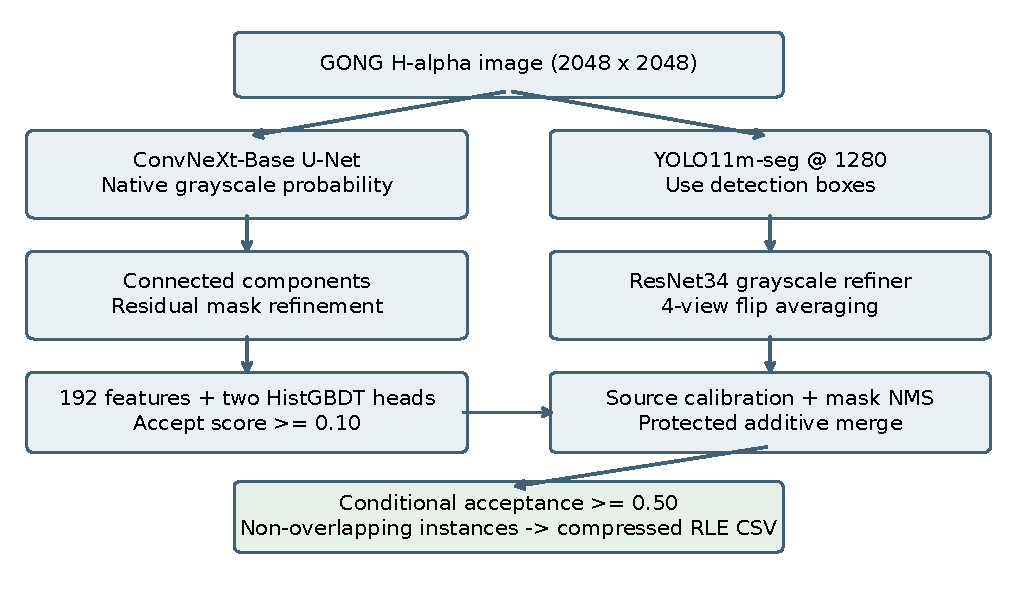
\includegraphics[width=\linewidth]{pipeline.pdf}
\caption{Frozen inference pipeline. The Base branch uses native full-image probabilities. The detector branch is additive: accepted Base instance masks are never overwritten. Conditional filtering occurs after painting, without reclaiming pixels from rejected supplements.}
\Description{Two inference branches join through an overlap-protected additive merge to generate an RLE CSV.}
\end{figure}

The retained detector branch is the historical A-cohort model: 451 training images, 57 selection images, and 57 source-calibration images, all within that cohort's 565-image training side. Conditional calibration uses 190 training-side OOF images. Thus, ``707-image Base'' does not mean that every component was fitted on 707 images. The supplied detector and grayscale-refiner weights are retained exactly; no full-data detector refit is substituted.

\subsection{Dense foreground and native candidates}
The Base uses a ConvNeXt-Base encoder \cite{convnext} and U-Net decoder \cite{unet}, implemented with Segmentation Models PyTorch. The decoder widths are 256, 128, 64, 32, and 16. Grayscale input is normalized as $(I/255-0.5)/0.25$. The ImageNet stem is adapted to grayscale while accounting for RGB normalization. Training uses native $512\times512$ crops, batch size 4, and 72 epochs of 128 updates (9,216 updates). Sampling selects an annotated object's jittered center with probability 0.75, otherwise a random crop. Augmentation comprises right-angle rotations, horizontal flips, contrast scaling in $[0.9,1.1]$, and brightness offsets in $[-0.03,0.03]$.

The foreground loss is positive-weighted binary cross-entropy (weight 5) plus soft Dice. AdamW uses weight decay 0.01 and the frozen encoder/decoder learning-rate schedule: a 256-update warm-up to $5\!\times\!10^{-5}$/$2\!\times\!10^{-4}$, followed by the recorded schedule. The final exponential-moving-average weights are deployed, with maximum decay 0.999. The full schedule is included in the training recipe manifest.

Inference is a single native $2048\times2048$ Base forward pass, with BF16 autocast and float32 sigmoid probabilities $p$. Eight-connected components of $p\geq0.35$ are retained if their area is at least 50 pixels and peak probability is at least 0.75. There is no Base test-time augmentation, multiseed averaging, or learned affinity head in this submission.

\subsection{Instance refinement and quality filtering}
Each component is refined by a small residual U-Net using grayscale intensity, Base probability, and the component seed. Its encoder widths are 16/32/64/128, with GroupNorm and SiLU blocks. Native $256\times256$ patches cover the component with a 64-pixel margin and 128-pixel stride. Overlapping patch probabilities are blended using a Hann window floored at 0.05. The refiner adds a fixed seed-logit prior. Thresholded foreground must touch its seed and remain within 64 pixels of it. No resizing is used in this Base refinement branch.

The refiner is trained from scratch for 39 epochs of 128 updates with batch size 8, learning rate $3\!\times\!10^{-4}$, and weight decay $10^{-4}$. Its expert-aware BCE/Dice objective downweights annotator-disagreement pixels to 0.25. Quality filtering follows refinement; pixel ownership is resolved only among accepted instances, using the highest refinement probability. Exact ties preserve the earlier candidate.

For each original/refined candidate, we extract 192 features: 17 morphology/intensity descriptors, a variant indicator, spatial means and standard deviations at $1\times1$, $2\times2$, and $4\times4$, and mask/ring/edge appearance summaries. The feature crop has intensity, Base-probability, and candidate-mask channels, resized to $96\times96$. Two histogram gradient-boosted regressors \cite{sklearn} are trained on 17,676 OOF candidate rows. Targets are the mean best IoU and the fraction of experts for whom best IoU exceeds 0.5; experts are not merged into a union target.

Both trees use squared error, 200 iterations, learning rate 0.05, maximum depth 4, at most 15 leaves, minimum leaf size 30, L2 regularization 10, and no early stopping. Outputs are clipped to $[0,1]$. A refined candidate is accepted when
\begin{equation}
q(c)=\widehat{\operatorname{IoU}}(c)\,\widehat{\Pr(\operatorname{IoU}>0.5)}(c)\geq0.10.
\end{equation}
The two regressions are quality surrogates, not a claim of perfectly calibrated probabilities. They filter candidates without changing their predicted geometry.

\subsection{Protected detector supplements}
YOLO11m-seg \cite{yolo11} runs at input size 1280 with confidence floor 0.05. The pipeline uses its bounding boxes, rather than directly exporting its low-resolution masks. A separate ImageNet-initialized ResNet34 U-Net predicts a grayscale crop mask. The crop side is 1.8 times the longest box dimension, with minimum 96 pixels, resized to 256. This refiner was trained for 15 epochs using mask and annotated-spine supervision; the detector ran for 40 epochs, with checkpoint selection restricted to the 57-image selection subset.

Crop inference averages identity, horizontal, vertical, and double-flip predictions in FP32. If the thresholded area ratio of the average to identity falls outside $[0.60,1.70]$, identity is used instead. Probabilities are quantized to uint8 before bilinear restoration to native crop size, then thresholded strictly above 0.5. These numerical details are preserved from the credited community implementation \cite{community}.

Frozen piecewise-linear source calibration retains scores at least 0.5, followed by whole-mask NMS at IoU 0.05 and descending-score painting. A supplement with IoU above 0.05 against any Base mask is blocked. Otherwise, already occupied pixels are removed and at least 20 pixels must remain. Finally, the frozen conditional map must return at least 0.5. This last rejection does not trigger repainting. Consequently, all Base masks survive fusion unchanged, but additive false positives remain possible.


\begin{table}[h]
\caption{Frozen deployment components. OOF models are used during training; only these five files are loaded for test inference. Sizes include saved metadata.}
\centering\small
\begin{tabular}{lrr}\toprule
Component & Fit images & File (MiB)\\\midrule
ConvNeXt-Base U-Net & 707 & 353.62\\
Residual refiner & 707 OOF & 2.17\\
Two-head HistGBDT & 707 OOF & 1.21\\
YOLO11m-seg & 451 & 43.24\\
ResNet34 crop refiner & 451 & 93.36\\\bottomrule
\end{tabular}
\end{table}

\clearpage
\section{Evaluation}\label{sec:evaluation}
\subsection{Protocol and local results}
We evaluate complete masks using official float32 IoU matrices with strict IoU $>0.5$ matching, independently for each expert. PQ is aggregated from IoU sum $S$ and counts:
\begin{equation}
\operatorname{PQ}=S/(TP+0.5FP+0.5FN).
\end{equation}
No Hungarian replacement of the official matching rule is used. Small objects have area below 500 native pixels; faint objects use the frozen local contrast criterion: the median intensity in the GT dilation ring (radii 2 to 8 pixels), minus the median inside the GT, is below 16 grayscale levels. These subgroups describe evaluation, not test-time selection.

Table~\ref{tab:ab} reports recipe-matched isolated models, each trained on 565 images and evaluated on 142 held images. A has 246 expert sets and B has 227. Each uses its own excluded-data models and calibration maps. These are historical, repeatedly inspected holdouts with overlapping training populations, not a new blind test or an independent evaluation of the 707-image deployment weights.

\begin{table}[t]
\caption{Historical complete-pipeline evaluation. ``Base'' includes residual refinement and tree filtering. ``+YOLO'' is the protected supplement. Counts sum separate expert evaluations.}
\label{tab:ab}\centering\small
\begin{tabular}{llrrrr}\toprule
Split & Pipeline & PQ & TP & FP & FN\\\midrule
A & Base & .45098 & 1150 & 579 & 596\\
A & +YOLO & .45241 & 1163 & 597 & 583\\
B & Base & .45167 & 1129 & 598 & 549\\
B & +YOLO & .45183 & 1136 & 612 & 542\\\bottomrule
\end{tabular}
\end{table}

In A, the supplement adds 13 matches and 18 false positives; in B, it adds 7 matches and 14 false positives. Old Base matches are preserved. Small-object matches increase from 108 to 111 of 240 in A and from 125 to 128 of 270 in B. Faint matches increase from 455 to 462 of 865 and from 379 to 383 of 732, respectively. These are modest recall gains, not evidence that additional candidates are uniformly beneficial.

We use 10,000 date-cluster bootstrap resamples (seed 20261113). The 95\% interval for complete PQ is 0.43481 to 0.47018 in A, and 0.43158 to 0.47235 in B. For the paired supplement gain, the intervals are -0.00054 to 0.00373 in A, and -0.00146 to 0.00195 in B. Both include zero. This fixed-model bootstrap does not cover training randomness, prior model selection, or repeated use of the holdouts; A and B are not treated as independent replications.

\begin{figure}[t]
\centering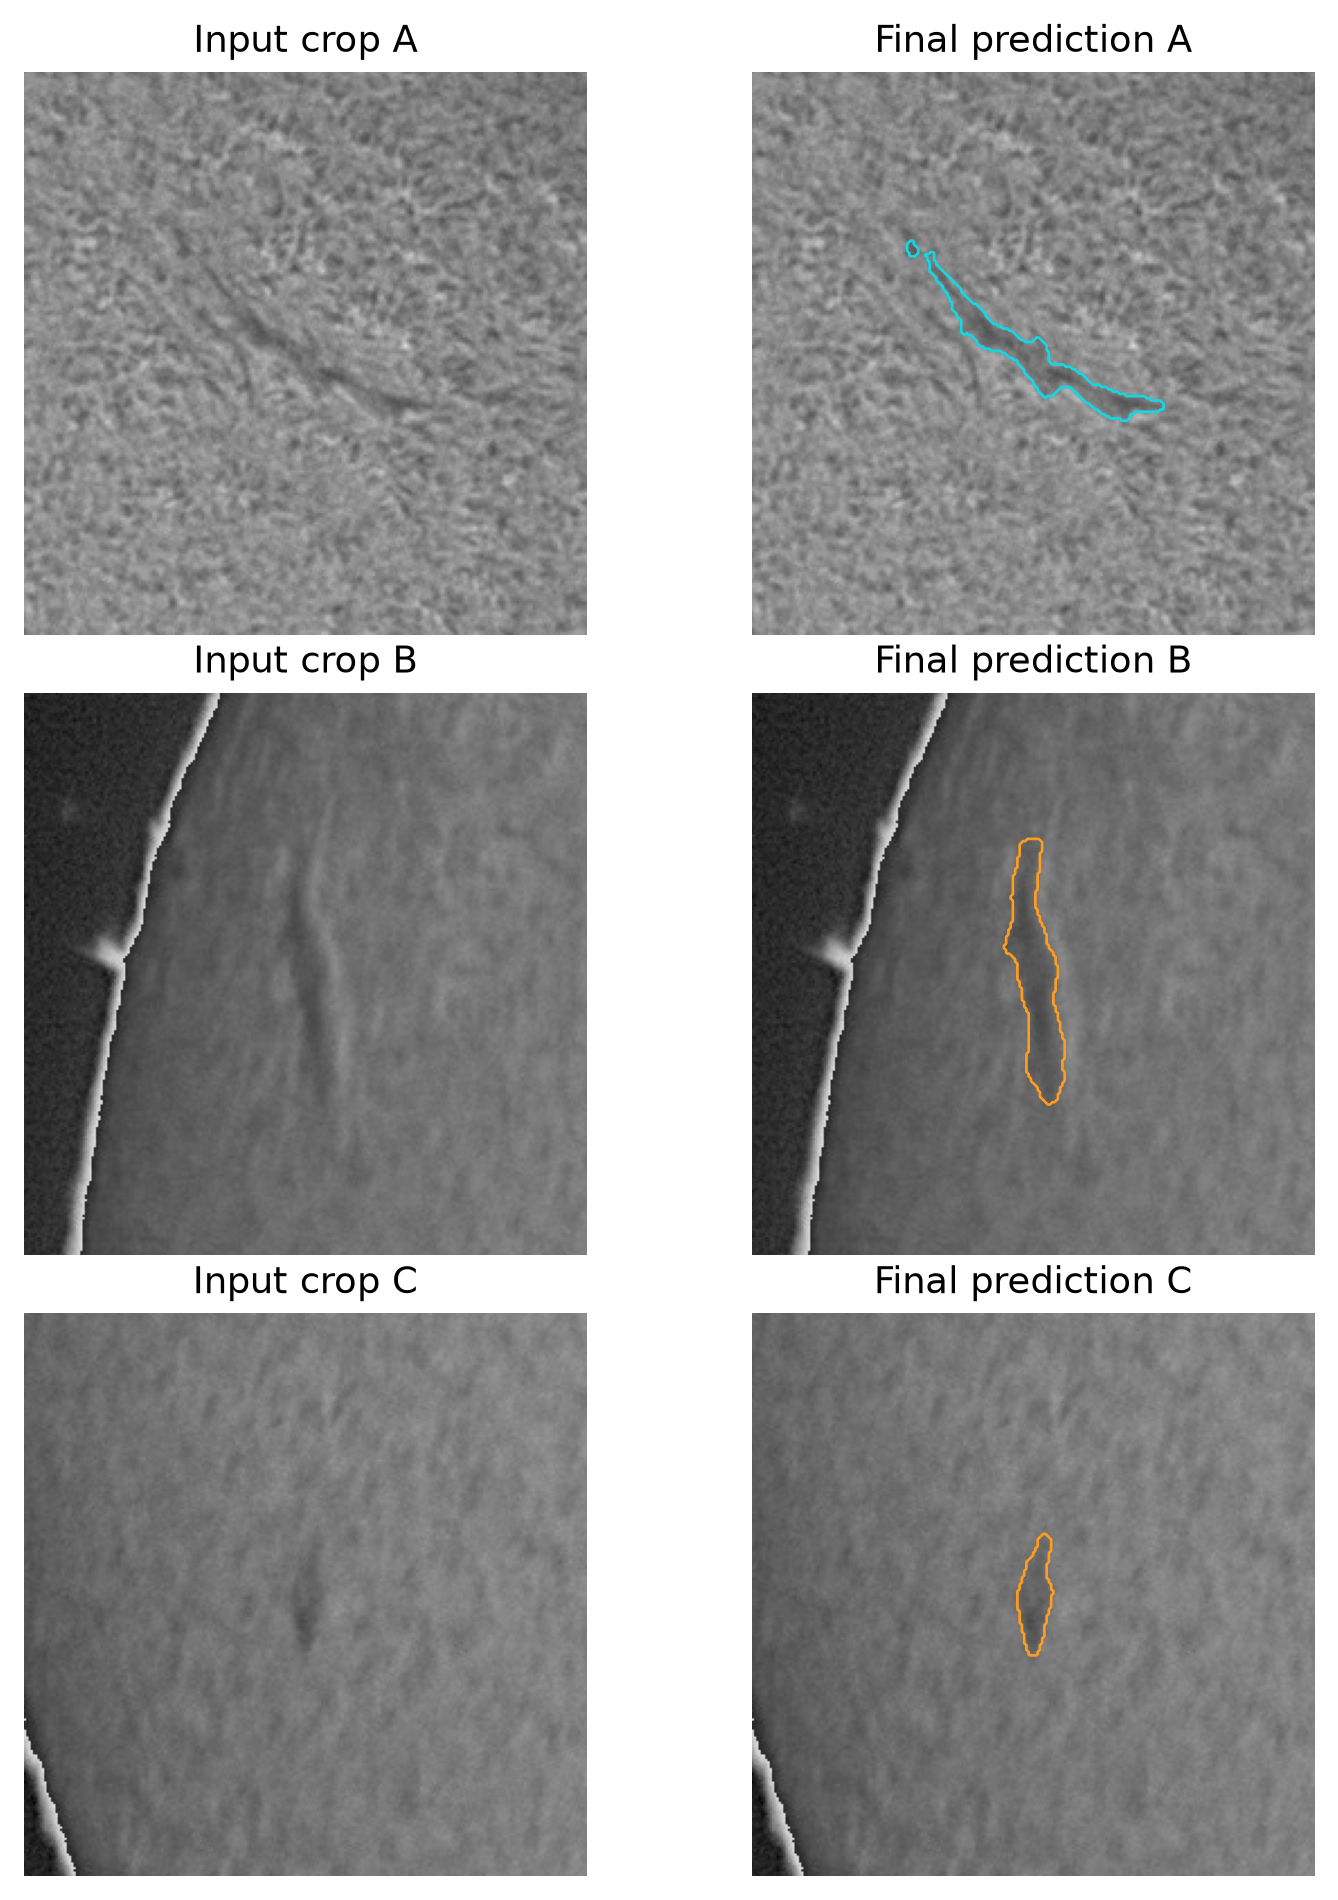
\includegraphics[width=\linewidth]{examples.png}
\caption{Prediction-only test-image crops. Cyan outlines are accepted Base instances; orange outlines are detector supplements. The first Base instance in frozen test order is shown, followed by the first supplement in each of the first two images containing a supplement. No GT was used for selection. These visualizations do not establish correctness or test recall.}
\Description{Three input crops alongside corresponding cyan and orange predicted instance outlines.}
\end{figure}

\subsection{Submitted result and limitations}
The retained CSV contains 1,220 Base instances and 41 supplements on 180 images. Its public leaderboard display was reported as 0.40. The exact unrounded score and private result are unavailable. Public values rounded to two decimals should not be interpreted as exact effect sizes. No local PQ is assigned to the actual 707-image weights. Later tested alternatives were not silently substituted into this submission.

Remaining errors include missed small and faint objects, merged connected components, refinement-induced geometry errors, and quality-score shift between OOF and deployment candidates. Quality filtering cannot recover an object that is absent from the candidate pool. Protected merging avoids damage to accepted Base masks but cannot resolve an existing Base merge or guarantee that a new instance is correct. Our local supplement confidence intervals include zero. Future improvements therefore require complete-pipeline evaluation rather than optimizing raw recall or a classifier metric alone.

\clearpage
\balance
\section{Reproducibility}
The public reproduction repository\footnote{\url{https://github.com/Lipeilin0307/filament-segmentation-2026}} contains five frozen model files (approximately 494 MiB), exact calibration arrays, source provenance, version-pinned dependencies, and an end-to-end inference Notebook. The Notebook starts with the official test images and regenerates both branches. It needs no training annotations, historical predictions, probability caches, or retraining. Models are constructed without automatic pretrained-weight downloads. The supplied pickle/checkpoints are hash-checked before deserialization.

Verification is separate from inference: it checks image coverage, consecutive instance IDs, nonempty and disjoint masks, RLE round-trip identity, and exact agreement with the retained submission. The reference CSV is read only after predictions have been generated. The verified target SHA256 is recorded in the package manifest. Both the command-line run and the executed Notebook regenerated all 180 images and reproduced the exact CSV bytes. In this session they took 314.6 and 672.3 seconds, respectively, on an RTX 5090. Both recorded 2.20 GiB peak PyTorch allocation; this excludes driver and cache memory. The manifests retain these measurements. Numerical reproduction is validated on Windows with the pinned CUDA stack; bit identity on other hardware or package versions is not assumed.

The detector crop-refinement routines are attributed to the public community repository at commit \texttt{84c9c7ca0523} \cite{community}; the report does not claim those routines or the underlying architectures as original. Anonymous repository and model downloads were verified on November 14, 2026. Third-party attribution and unresolved licensing status are documented separately; numerical parity does not establish license clearance.

\section{Acknowledgment}\label{sec:acknowledgment}
    % Do not change
    The organization of the Filament Segmentation Challenge 2026 is partially supported by the U.S. National Science Foundation (NSF) under Grant No. 2209912 and 2433781, directorate for Computer and Information Science and Engineering (CSE), and Office of Advanced Cyberinfrastructure (OAC), and Grant No. 2511630, AST Division Of Astronomical Sciences and MPS Directorate for Mathematical and Physical Sciences.

    The Filament Segmentation Challenge 2026 is sponsored by the U.S. National Science Foundation (NSF) National Solar Observatory (NSO). 

    This work utilizes GONG data obtained by the NSO Integrated Synoptic Program, managed by the National Solar Observatory, which is operated by the Association of Universities for Research in Astronomy (AURA), Inc. under a cooperative agreement with the National Science Foundation and with contribution from the National Oceanic and Atmospheric Administration. The GONG network of instruments is hosted by the Big Bear Solar Observatory, High Altitude Observatory, Learmonth Solar Observatory, Udaipur Solar Observatory, Instituto de Astrofísica de Canarias, and Cerro Tololo Interamerican Observatory.


\bibliographystyle{ACM-Reference-Format}
\bibliography{main}
\end{document}
